%  LaTeX support: latex@mdpi.com
%  In case you need support, please attach all files that are necessary for compiling as well as the log file, and specify the details of your LaTeX setup (which operating system and LaTeX version / tools you are using).

%=================================================================
\documentclass[water,article,submit,moreauthors,pdftex]{mdpi}

% If you would like to post an early version of this manuscript as a preprint, you may use preprint as the journal and change 'submit' to 'accept'. The document class line would be, e.g., \documentclass[preprints,article,accept,moreauthors,pdftex]{mdpi}. This is especially recommended for submission to arXiv, where line numbers should be removed before posting. For preprints.org, the editorial staff will make this change immediately prior to posting.

%% Some pieces required from the pandoc template
\setlist[itemize]{leftmargin=*,labelsep=5.8mm}
\setlist[enumerate]{leftmargin=*,labelsep=4.9mm}


%--------------------
% Class Options:
%--------------------
%----------
% journal
%----------
% Choose between the following MDPI journals:
% acoustics, actuators, addictions, admsci, aerospace, agriculture, agriengineering, agronomy, algorithms, animals, antibiotics, antibodies, antioxidants, applsci, arts, asc, asi, atmosphere, atoms, axioms, batteries, bdcc, behavsci , beverages, bioengineering, biology, biomedicines, biomimetics, biomolecules, biosensors, brainsci , buildings, cancers, carbon , catalysts, cells, ceramics, challenges, chemengineering, chemistry, chemosensors, children, cleantechnol, climate, clockssleep, cmd, coatings, colloids, computation, computers, condensedmatter, cosmetics, cryptography, crystals, dairy, data, dentistry, designs , diagnostics, diseases, diversity, drones, econometrics, economies, education, electrochem, electronics, energies, entropy, environments, epigenomes, est, fermentation, fibers, fire, fishes, fluids, foods, forecasting, forests, fractalfract, futureinternet, futurephys, galaxies, games, gastrointestdisord, gels, genealogy, genes, geohazards, geosciences, geriatrics, hazardousmatters, healthcare, heritage, highthroughput, horticulturae, humanities, hydrology, ijerph, ijfs, ijgi, ijms, ijns, ijtpp, informatics, information, infrastructures, inorganics, insects, instruments, inventions, iot, j, jcdd, jcm, jcp, jcs, jdb, jfb, jfmk, jimaging, jintelligence, jlpea, jmmp, jmse, jnt, jof, joitmc, jpm, jrfm, jsan, land, languages, laws, life, literature, logistics, lubricants, machines, magnetochemistry, make, marinedrugs, materials, mathematics, mca, medicina, medicines, medsci, membranes, metabolites, metals, microarrays, micromachines, microorganisms, minerals, modelling, molbank, molecules, mps, mti, nanomaterials, ncrna, neuroglia, nitrogen, notspecified, nutrients, ohbm, particles, pathogens, pharmaceuticals, pharmaceutics, pharmacy, philosophies, photonics, physics, plants, plasma, polymers, polysaccharides, preprints , proceedings, processes, proteomes, psych, publications, quantumrep, quaternary, qubs, reactions, recycling, religions, remotesensing, reports, resources, risks, robotics, safety, sci, scipharm, sensors, separations, sexes, signals, sinusitis, smartcities, sna, societies, socsci, soilsystems, sports, standards, stats, surfaces, surgeries, sustainability, symmetry, systems, technologies, test, toxics, toxins, tropicalmed, universe, urbansci, vaccines, vehicles, vetsci, vibration, viruses, vision, water, wem, wevj

%---------
% article
%---------
% The default type of manuscript is "article", but can be replaced by:
% abstract, addendum, article, benchmark, book, bookreview, briefreport, casereport, changes, comment, commentary, communication, conceptpaper, conferenceproceedings, correction, conferencereport, expressionofconcern, extendedabstract, meetingreport, creative, datadescriptor, discussion, editorial, essay, erratum, hypothesis, interestingimages, letter, meetingreport, newbookreceived, obituary, opinion, projectreport, reply, retraction, review, perspective, protocol, shortnote, supfile, technicalnote, viewpoint
% supfile = supplementary materials

%----------
% submit
%----------
% The class option "submit" will be changed to "accept" by the Editorial Office when the paper is accepted. This will only make changes to the frontpage (e.g., the logo of the journal will get visible), the headings, and the copyright information. Also, line numbering will be removed. Journal info and pagination for accepted papers will also be assigned by the Editorial Office.

%------------------
% moreauthors
%------------------
% If there is only one author the class option oneauthor should be used. Otherwise use the class option moreauthors.

%---------
% pdftex
%---------
% The option pdftex is for use with pdfLaTeX. If eps figures are used, remove the option pdftex and use LaTeX and dvi2pdf.

%=================================================================
\firstpage{1}
\makeatletter
\setcounter{page}{\@firstpage}
\makeatother
\pubvolume{xx}
\issuenum{1}
\articlenumber{5}
\pubyear{2019}
\copyrightyear{2019}
%\externaleditor{Academic Editor: name}
\history{Received: date; Accepted: date; Published: date}
\updates{yes} % If there is an update available, un-comment this line

%% MDPI internal command: uncomment if new journal that already uses continuous page numbers
%\continuouspages{yes}

%------------------------------------------------------------------
% The following line should be uncommented if the LaTeX file is uploaded to arXiv.org
%\pdfoutput=1

%=================================================================
% Add packages and commands here. The following packages are loaded in our class file: fontenc, calc, indentfirst, fancyhdr, graphicx, lastpage, ifthen, lineno, float, amsmath, setspace, enumitem, mathpazo, booktabs, titlesec, etoolbox, amsthm, hyphenat, natbib, hyperref, footmisc, geometry, caption, url, mdframed, tabto, soul, multirow, microtype, tikz

%=================================================================
%% Please use the following mathematics environments: Theorem, Lemma, Corollary, Proposition, Characterization, Property, Problem, Example, ExamplesandDefinitions, Hypothesis, Remark, Definition
%% For proofs, please use the proof environment (the amsthm package is loaded by the MDPI class).

%=================================================================
% Full title of the paper (Capitalized)
\Title{Calibration, Validation, and Radiation\(:\) Predicting Biogenic
Silica and Organic Carbon Percentages in Lake Sediment Core Samples}

% Authors, for the paper (add full first names)
\Author{Rana
Gahwagy$^{1}$\href{https://orcid.org/0000-0003-3293-2315}{\orcidicon}, Lauren
Meyer$^{1}$, Grace Hartley$^{1}$}

% Authors, for metadata in PDF
\AuthorNames{Rana Gahwagy, Lauren Meyer, Grace Hartley}

% Affiliations / Addresses (Add [1] after \address if there is only one affiliation.)
\address{%
$^{1}$ \quad Smith College Department of Statistical and Data Sciences
Northampon, MA 01063; \\
}
% Contact information of the corresponding author
\corres{Correspondence: }

% Current address and/or shared authorship








% The commands \thirdnote{} till \eighthnote{} are available for further notes

% Simple summary

% Abstract (Do not insert blank lines, i.e. \\)
\abstract{In many settings, biogenic silica (BSi) and total organic
carbon (TOC) are widely used as proxies for temperature and/or
environmental variations that are helpful in paleoclimate and
paleoenvironmental reconstructions. Often, the methodology for analyzing
these parameters in sediments can be expensive and time consuming
(particularly for BSi). However, Fourier Transform Infrared (FTIR)
Spectroscopy offers an efficient alternative where many samples can be
run with minimal amount of sediment and time. This technique is
advantageous in that it requires small volumes of sediment
(\textasciitilde0.01g), minimal sample preparation (mixing sample with
potassium bromide powder), and instrumental analysis times are
relatively rapid (a few minutes per sample). FTIR Spectroscopy
quantifies BSi and TOC using infrared radiation (IR) absorbance
units---as opposed to percentages of BSi or TOC---which are difficult to
compare across different studies and localities. Therefore, there is a
need for a systematic way to convert the results from the FTIR
Spectrometer into percentages. In this research project, we address this
need by building a universal calibration model using partial least
squares (PLS) regression that converts BSi absorbance to percentages. We
developed this model using a PLS package in R and based our model on
samples from Arctic lakes in Greenland and Alaska. Our preliminary model
uses a k-fold cross-validation method and utilizes three components.
Ongoing work intends to improve on the model's prediction accuracy,
expand our calibration model to include TOC percentages, and incorporate
more BSi samples from other locations. We aim for the model to be
universal and integrated into a Shiny app, where paleoclimatologists can
use it on samples from various localities and compare their results.
This model will prove a valuable tool in paleoclimate reconstruction by
facilitating FTIR Spectroscopy on lake sediments.}

% Keywords

% The fields PACS, MSC, and JEL may be left empty or commented out if not applicable
%\PACS{J0101}
%\MSC{}
%\JEL{}

%%%%%%%%%%%%%%%%%%%%%%%%%%%%%%%%%%%%%%%%%%
% Only for the journal Diversity
%\LSID{\url{http://}}

%%%%%%%%%%%%%%%%%%%%%%%%%%%%%%%%%%%%%%%%%%
% Only for the journal Applied Sciences:
%\featuredapplication{Authors are encouraged to provide a concise description of the specific application or a potential application of the work. This section is not mandatory.}
%%%%%%%%%%%%%%%%%%%%%%%%%%%%%%%%%%%%%%%%%%

%%%%%%%%%%%%%%%%%%%%%%%%%%%%%%%%%%%%%%%%%%
% Only for the journal Data:
%\dataset{DOI number or link to the deposited data set in cases where the data set is published or set to be published separately. If the data set is submitted and will be published as a supplement to this paper in the journal Data, this field will be filled by the editors of the journal. In this case, please make sure to submit the data set as a supplement when entering your manuscript into our manuscript editorial system.}

%\datasetlicense{license under which the data set is made available (CC0, CC-BY, CC-BY-SA, CC-BY-NC, etc.)}

%%%%%%%%%%%%%%%%%%%%%%%%%%%%%%%%%%%%%%%%%%
% Only for the journal Toxins
%\keycontribution{The breakthroughs or highlights of the manuscript. Authors can write one or two sentences to describe the most important part of the paper.}

%\setcounter{secnumdepth}{4}
%%%%%%%%%%%%%%%%%%%%%%%%%%%%%%%%%%%%%%%%%%


% tightlist command for lists without linebreak
\providecommand{\tightlist}{%
  \setlength{\itemsep}{0pt}\setlength{\parskip}{0pt}}

% From pandoc table feature
\usepackage{longtable,booktabs,array}
\usepackage{calc} % for calculating minipage widths
% Correct order of tables after \paragraph or \subparagraph
\usepackage{etoolbox}
\makeatletter
\patchcmd\longtable{\par}{\if@noskipsec\mbox{}\fi\par}{}{}
\makeatother
% Allow footnotes in longtable head/foot
\IfFileExists{footnotehyper.sty}{\usepackage{footnotehyper}}{\usepackage{footnote}}
\makesavenoteenv{longtable}



\begin{document}


%%%%%%%%%%%%%%%%%%%%%%%%%%%%%%%%%%%%%%%%%%

\hypertarget{introduction}{%
\section{Introduction}\label{introduction}}

Studying the content of biogenic silica and other organic compounds
present in lake sediment cores can be a powerful tool in gaining insight
into our reconstruction of past climates. The wet chemistry processes
used to determine these proportions can be time consuming and costly. As
a result, data on the amount of biogenic silica present in different
samples is limited in quantity and resolution. Fourier-transform
infrared (FTIR) spectroscopy is a promising technique to reduce the time
and money needed to determine the proportion of these compounds in lake
sediments. FTIR spectroscopy involves measuring the absorbance of the
infrared radiation at different wavelengths. These absorbance values are
arbitrary and unitless \citep{kamat2013make}, so interpretation is
needed to make them relevant between researchers. To interpret these
absorbance values, we seek to use a Partial Least Squares Regression
(PLSR) model to predict the percentage of the biogenic silica in each
sample. This technique has been pioneered successfully by
\citet{vogel2008fourier}, but is not accessible to those who might wish
to use FTIR spectroscopy for their samples and lack the statistical
background to implement a PLSR model.

The goal of this project is to create an interface where a user can
input their FTIR spectroscopy data into a PLSR model to calculate the
approximate biogenic silica and total organic carbon percentages. Our
work primarily includes improving the accuracy of the existing model
(\url{https://github.com/people-r-strange/PLSmodel}) and preparing for
universal input. This includes selection of the most applicable
diagnostic plots to determine the accuracy of the model. Because this
work will be accessible to the public, our model and corresponding
interface satisfy an existing need for efficient FTIR spectroscopy
interpretation. Further, greater accessibility and use of this
technology may eliminate the need for expensive wet chemical processes.

\hypertarget{data}{%
\section{Data}\label{data}}

Our model is trained on spectroscopy data gathered from the analysis of
lake bed samples. 26 samples are from Greenland collected by Greg de
Wet, 103 are from Alaska collected by Daryl Kaufman at Northern Arizona
University, and samples of only diatoms and only washed quartz. Each
pre-processed dataset has two variables: wavenumbers tested, and
corresponding absorbance values measuring the sample's absorbance of
that specific wavenumber of light (Figure \ref{fig:fig1}). Each sample
also has a single associated measurement of biogenic silica, calculated
by traditional wet chemistry digestion methods.

\begin{verbatim}
## Warning: Removed 1814 row(s) containing missing values (geom_path).
\end{verbatim}

\begin{figure}

{\centering 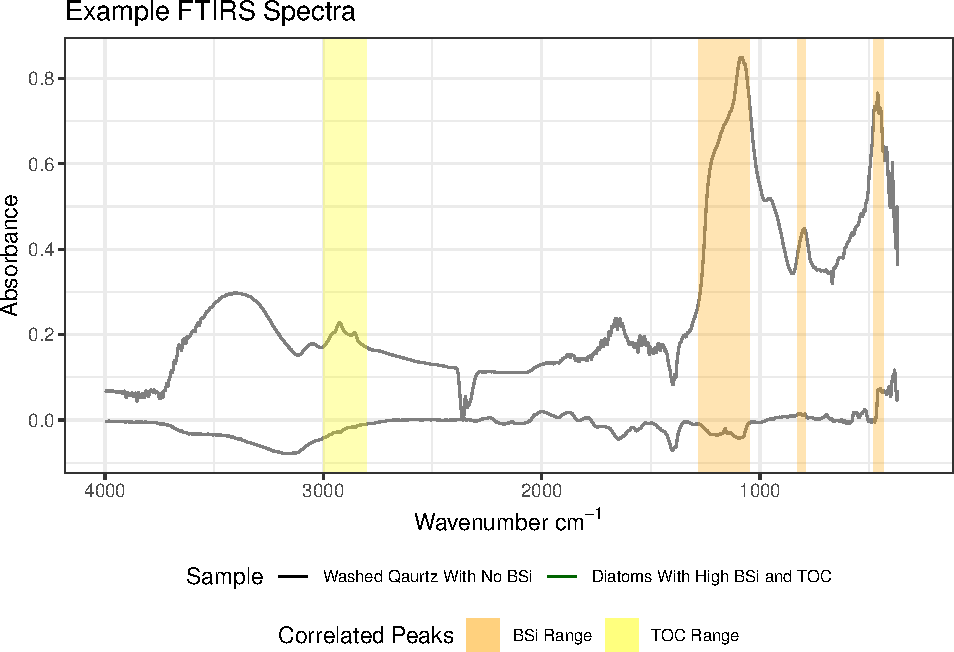
\includegraphics{final_paper_draft_files/figure-latex/fig1-1} 

}

\caption{Comparison between absorbance values across the spectrum of wavelength for two calibration samples, one of pure diatoms, which have high biogenic silica (BSi) and total organic carbon (TOC) content, and one of washed quartz which has no BSi or TOC. Highlighted areas are ranges that correlate with BSi (in orange) and TOC (in yellow). The area under those peaks is what is usually reported in literature.}\label{fig:fig1}
\end{figure}

\begin{figure}

{\centering 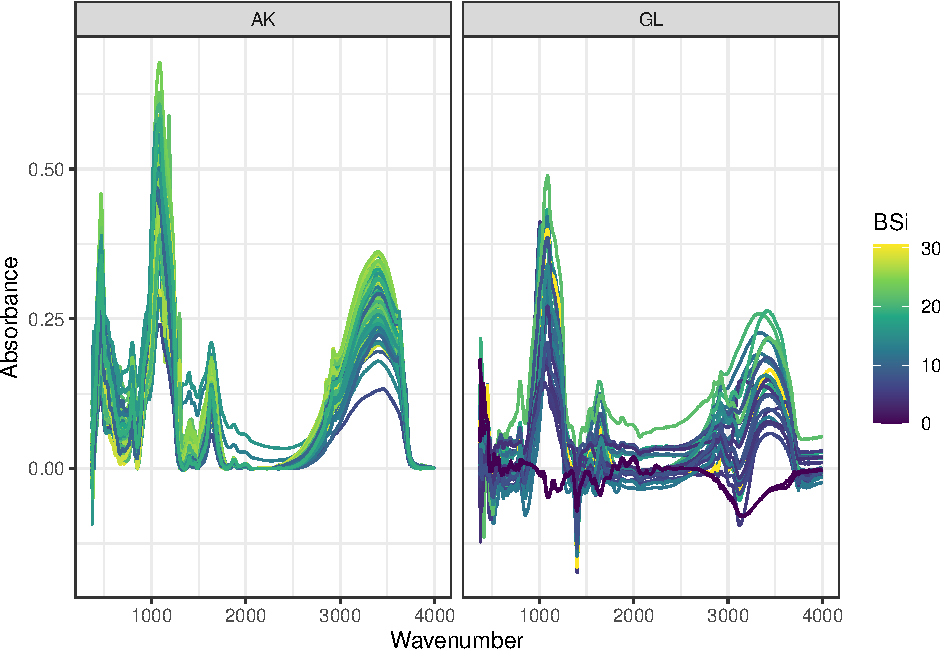
\includegraphics{final_paper_draft_files/figure-latex/fig2-1} 

}

\caption{Each sample’s spectrum is plotted here by region and color coded with actual biogenic silica (BSi) where dark blue colors are samples with low BSi and yellow denotes high BSi.}\label{fig:fig2}
\end{figure}

The Greenland samples were tested at 3,697 distinct wavenumbers, ranging
from 368 \(cm^{-1}\) to 7497 \(cm^{-1}\), while the Alaska samples were
tested at 1,882 distinct wavenumbers ranging from 368 cm\^{}\{-1\} to
3996 \(cm^{-1}\). The relationship between absorbance and wavenumber is
smooth for all samples between the wavenumbers of 500 \(cm^{-1}\) and
4000 \(cm^{-1}\), though below 500 \(cm^{-1}\) and above 4000
\(cm^{-1}\) the line shows increased noise, with the noise being the
worst at the highest wavenumbers. This is evident in figure
\ref{fig:fig2}, and even more notably in the higher wavenumbers of the
wet quartz data in figure \ref{fig:fig3}.

The Greenland samples and the Alaskan samples were analyzed at different
times with slightly different spectroscopy settings, so the wavenumbers
measured do not match exactly. Even though the difference is small, the
regression model requires the wavenumber labels to be consistent as they
are the explanatory variables in the model. In addition, the Alaskan
samples were analyzed on a much smaller range of wavenumbers than the
Greenland samples, though the resolution was about the same. Therefore,
the two sets of data have a mismatch in the number of columns, which we
resolve using linear interpolation and elaborate below.

\begin{figure}

{\centering 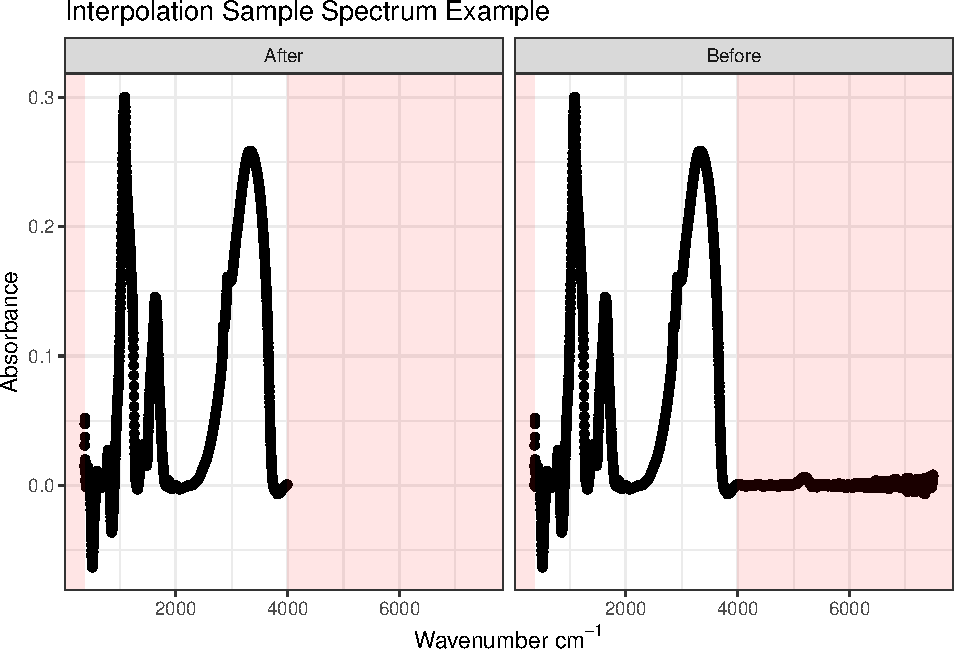
\includegraphics{final_paper_draft_files/figure-latex/fig3-1} 

}

\caption{A closer look at the Absorbance spectrum of a random sample from Greenland shows that the raw data (Before) has a lot of noise in wavenumbers above 4000 $cm^{-1}$, which is consistent throughout all samples. After truncating the spectrum and interpolating the Greenland data (After) there were negligible changes.}\label{fig:fig3}
\end{figure}

\hypertarget{methods}{%
\section{Methods}\label{methods}}

We use functions from the \texttt{pls} R package to create and evaluate
our PLSR models \citep{R-pls}. The original model was created using this
same package. In order to run the PLSR model, we need all datasets to
include the same amount of wavenumber columns with identical labels.
This is because each wavenumber is treated as an independent variable in
the model, and prediction is not possible if each sample has slightly
different independent variables.

In order to solve this issue, we will linearly interpolate the
absorbance spectrum from each Greenland sample to match the wavenumbers
of the Alaskan samples, rounded to the nearest integer for ease of human
interpretation. This is because the range of wavenumbers measured in the
Alaskan samples is smaller, therefore interpolating Alaskan samples onto
the Greenland spectra would not be possible. Since the absorbance
spectra from both samples are high resolution and the differences
between the original and the interpolated absorbance values are small,
we are comfortable that this does not meaningfully alter the data.

The original model was trained on only the Greenland samples (n = 28) to
predict BSi content within the Greenland samples. To improve accuracy of
the model, we integrate the Alaskan samples (n =103). In total, we built
five different models to gauge the best performance with our data.

The first two models are region-specific; this includes the original
Greenland model mentioned above, as well as a similar model that uses
the Alaskan samples only. The next model uses the full spectrum of
combined Greenland and Alaska samples. The last two models use sections
of the combined Greenland and Alaskan spectra that are typically
correlated with high BSi content. One of the two models includes the
most reported peak between 1050-1280 \(cm^{-1}\), and the other
considers all associated peaks between 1050-1280 \(cm^{-1}\), 790 - 830
\(cm^{-1}\), and 435 - 480 \(cm^{-1}\) as highlighted in figure
\ref{fig:fig1} \citep{rosen2011universally}.

To compare the accuracy of these models, we look at the Mean Square
Error (MSE) and Mean Absolute Deviation (MAD) values from each model. We
employ assessment tools to determine the optimal number of components,
notably Root Mean Squared Error of Prediction (RMSEP). These values are
useful, because they are a simple, comparable metric. A good model will
minimize the size of prediction errors, leading to a small RMSEP.

\hypertarget{results}{%
\section{Results}\label{results}}

Comparing the different models based on the metrics mentioned above, we
find that the model that is trained on the full spectrum of the combined
samples (Greenland + Alaskan) predicts BSi content the best. This is
visible in table \ref{tab:tab1}, where we see that the combined full
spectrum model has a Mean Squared Error of 6.84, which is considerably
lower than even the next best model that has an MSE of 12.33.

\begin{longtable}[]{@{}llll@{}}
\caption{Overview of the five different models tested against each data
set. The Mean Square Error (MSE) and Mean Absolute Deviation (MAD) were
calculated to compare and the model that uses both the Alaska and
Greenland full spectrum shows optimal results.}\tabularnewline
\toprule
Data Trained On & Data Tested On & MSE & MAD \\
\midrule
\endfirsthead
\toprule
Data Trained On & Data Tested On & MSE & MAD \\
\midrule
\endhead
Greenland & Alaska & 61.78174700958 & 6.97577898211303 \\
Greenland & Combined & 47.0020588160737 & 5.64642471647423 \\
NA & NA & NA & NA \\
NA & Combined & NA & NA \\
NA & Combined & NA & NA \\
NA & Combined & NA & NA \\
NA & Combined & NA & NA \\
\bottomrule
\end{longtable}

Once we have the most appropriate model, we must choose how many
principal components to include within the model. Principal components
refer to latent variables that the algorithm predicts within the model
to use for prediction of the desired outcome variable (pls package
citation). Including too few principal components will not provide
enough predictive power, but too many risks an overly complex or
overfitted model. We look at a plot (figure \ref{fig:fig4}) of RMSEP
values for each potential number of components (n = 10), and find that
using 10 components creates a model with the lowest RMSEP. Despite the
high number of components, our model does not appear to overfit our data
because it accurately generalizes to new data that was not included in
the training data. Overall, our final model can be represented as:
\(BSi = x_1 + x_2 + . . . + x_{1882} + b\) where the \(x_n\) variables
are the individual wavenumbers and \(b\) is the intercept.

\begin{figure}

{\centering 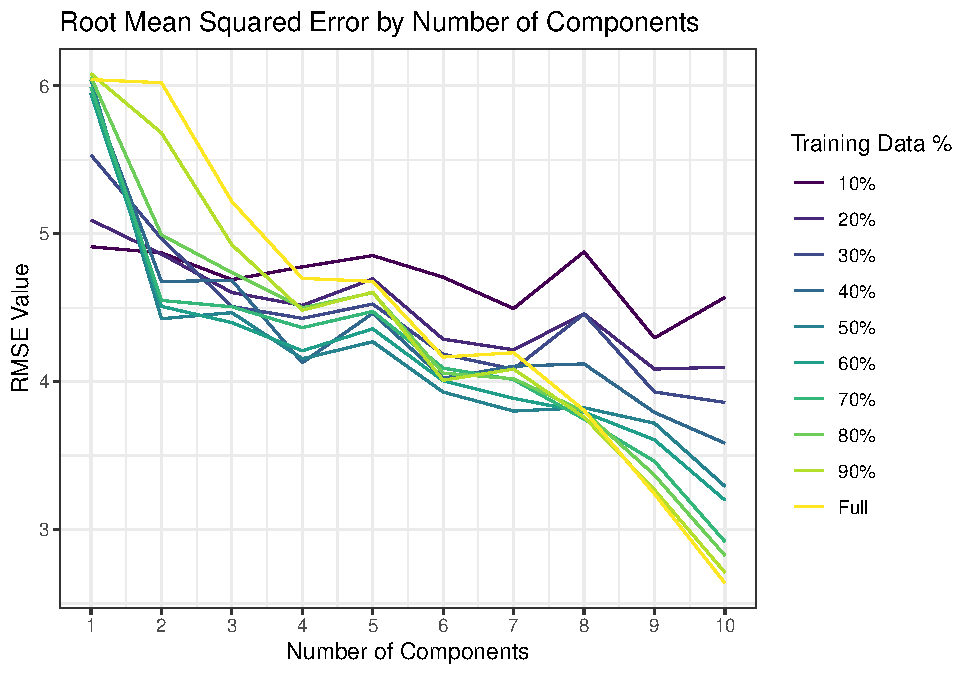
\includegraphics{final_paper_draft_files/figure-latex/fig4-1} 

}

\caption{The Root Mean Square Error of Prediction (RMSEP) was calculated against new data for each component. Ten random samples were taken of the data for each percentage, and the model trained on that sample was then tested against the remaining data for each component, with the values shown above being the mean of the ten iterations for each combination, to limit the variation inherent in sampling. Based on this, we chose the model with 10 components as our final model.}\label{fig:fig4}
\end{figure}

wordcountaddin::text\_stats()

% %%%%%%%%%%%%%%%%%%%%%%%%%%%%%%%%%%%%%%%%%%
% %% optional
% \supplementary{The following are available online at www.mdpi.com/link, Figure S1: title, Table S1: title, Video S1: title.}
%
% % Only for the journal Methods and Protocols:
% % If you wish to submit a video article, please do so with any other supplementary material.
% % \supplementary{The following are available at www.mdpi.com/link: Figure S1: title, Table S1: title, Video S1: title. A supporting video article is available at doi: link.}

\vspace{6pt}

%%%%%%%%%%%%%%%%%%%%%%%%%%%%%%%%%%%%%%%%%%

%%%%%%%%%%%%%%%%%%%%%%%%%%%%%%%%%%%%%%%%%%

%%%%%%%%%%%%%%%%%%%%%%%%%%%%%%%%%%%%%%%%%%

%%%%%%%%%%%%%%%%%%%%%%%%%%%%%%%%%%%%%%%%%%
%% optional
\abbreviations{The following abbreviations are used in this manuscript:\\

\noindent
\begin{tabular}{@{}ll}
FTIR & Fourier-Transform Infrared \\
PLSR & Partial Least Squares Regression \\
\end{tabular}}


%%%%%%%%%%%%%%%%%%%%%%%%%%%%%%%%%%%%%%%%%%
% Citations and References in Supplementary files are permitted provided that they also appear in the reference list here.

%=====================================
% References, variant A: internal bibliography
%=====================================
%\reftitle{References}
%\begin{thebibliography}{999}
% Reference 1
%\bibitem[Author1(year)]{ref-journal}
%Author1, T. The title of the cited article. {\em Journal Abbreviation} {\bf 2008}, {\em 10}, 142--149.
% Reference 2
%\bibitem[Author2(year)]{ref-book}
%Author2, L. The title of the cited contribution. In {\em The Book Title}; Editor1, F., Editor2, A., Eds.; Publishing House: City, Country, 2007; pp. 32--58.
%\end{thebibliography}

% The following MDPI journals use author-date citation: Arts, Econometrics, Economies, Genealogy, Humanities, IJFS, JRFM, Laws, Religions, Risks, Social Sciences. For those journals, please follow the formatting guidelines on http://www.mdpi.com/authors/references
% To cite two works by the same author: \citeauthor{ref-journal-1a} (\citeyear{ref-journal-1a}, \citeyear{ref-journal-1b}). This produces: Whittaker (1967, 1975)
% To cite two works by the same author with specific pages: \citeauthor{ref-journal-3a} (\citeyear{ref-journal-3a}, p. 328; \citeyear{ref-journal-3b}, p.475). This produces: Wong (1999, p. 328; 2000, p. 475)

%=====================================
% References, variant B: external bibliography
%=====================================
\reftitle{References}
\externalbibliography{yes}
\bibliography{mybibfile.bib}

%%%%%%%%%%%%%%%%%%%%%%%%%%%%%%%%%%%%%%%%%%
%% optional

%% for journal Sci
%\reviewreports{\\
%Reviewer 1 comments and authors’ response\\
%Reviewer 2 comments and authors’ response\\
%Reviewer 3 comments and authors’ response
%}

%%%%%%%%%%%%%%%%%%%%%%%%%%%%%%%%%%%%%%%%%%


\end{document}
